\chapter{Engenharia de Software}
\label{ch::engsoft}


\section{Introdução}
\label{sec::engsoft:intro}

% Um projeto de sucesso envolve uma preparação prévia exímia.
A plataforma \appname~desenvolvida pela \groupname~não foi exceção. Foram delineados antecipadamente vários pontos fulcrais, nomeadamente:

%TODO: I'm here <--

\begin{itemize}
    \item Ferramentas e tecnologias (Secção \ref{sec::engsoft:tecnologia}): perante uma equipa de 5 pessoas, foi vital determinar quais as tecnologias a utilizar não só para implementar a aplicação mas também para gerir o trabalho paralelo que iria decorrer;
    \item Requisitos funcionais e não-funcionais (Secção \ref{sec::engsoft:requisitos}): a aplicação deve cumprir uma série de requisitos a fim de poder alcançar os objetivos propostos;
    \item Diagramas de casos de uso (Secção \ref{sec::engsoft:casos-uso}): a fim de se perceber as atividades a desenhar e o respetivo código-fonte que as interliga, diferentes casos de uso foram estudados;
    \item Diagrama de atividades (Secção \ref{sec::engsoft:casos-uso}): este diagrama resume o fluxo de funcionamento da aplicação.
\end{itemize}


\section{Ferramentas e tecnologias utilizadas}
\label{sec::engsoft:tecnologia}

As ferramentas utilizadas no âmbito da realização do projeto, sumariadas na Tabela \ref{tab::ferramentas}, visam três componentes essenciais na sua gestão: 1) linguagem de programação, 2) servidor, 3) administração bd, 4) relatório, 5) controlo de versões.


\begin{table}[!htbp]
    \centering
    \begin{tabular}{p{1cm} l l}
        \toprule
        & {\itshape\bfseries Software} & {\bfseries Versão} \\
        \midrule
        \multicolumn{3}{l}{\bfseries Linguagem de Programação} \\
        & \textit{Python} & 3.8.0 \\
        \midrule
        \multicolumn{3}{l}{\bfseries Servidor} \\
        & \textit{Microsoft Windows Server} & 2019 \\
        & \textit{MariaDB} & 10.4.18 \\
        \midrule
        \multicolumn{3}{l}{\bfseries Administração BD} \\
        & \textit{DBeaver} & 21.0.5 \\
        \midrule
        \multicolumn{3}{l}{\bfseries Relatório} \\
        & \textit{Overleaf} & \\
        \midrule
        \multicolumn{3}{l}{\bfseries Controlo de versões} \\
        & \textit{git} & 2.17.1 \\
        & \textit{GitKraken} & 7.6.1  \\
        \midrule
        \bottomrule
    \end{tabular}
    \caption[Ferramentas utilizadas]{Ferramentas e tecnologias utilizadas, organizadas por categoria.}
    \label{tab::ferramentas}
\end{table}



\section{Requisitos}
\label{sec::engsoft:requisitos}

De forma a ir de encontro aos objetivos propostos do projeto (Secção \ref{sec::intro:descricao}), uma série de requisitos funcionais e não-funcionais foi delineada.

\subsection{Requisitos funcionais}
\label{ssec::engsoft:requisitos:funcionais}

A plataforma deve:

\begin{enumerate}
    \item Possuir um ecrã de boas-vindas e instruções de uso do sistema;
    \item Ter um ecrã de registo e \emph{login} de utilizadores;
    \item Ter uma \textit{homepage} com acesso direto às seguintes funcionalidades:
    \begin{enumerate}
        \item resolução de desafios disponíveis,
        \item propor desafios,
        \item pedir ajuda,
        \item \textit{scoreboard} dos utilizadores,
    \end{enumerate}
    \item Permitir responder a desafios;
    \item Permitir submeter dois tipos de desafios, em que um é de decifra de mensagem e outro de descoberta de mensagem.
\end{enumerate}


\subsection{Requisitos não-funcionais}
\label{ssec::engsoft:requisitos:nao-funcionais}

A plataforma deve:

\begin{enumerate}
    \item Permitir apenas uma tentiva a cada 15 segundos para os desafios cifrados;
    \item Usar assinaturas digitais \ac{RSA};
    \item Ter uma interface gráfica minimalista e (\textit{user-friendly});
    \item Ser segura em termos do armazenamento dos dados na base de dados (se possível cifrar os dados guardados duplamente no caso dos desafios).
\end{enumerate}


\section{Casos de Uso}
\label{sec::engsoft:casos-uso}

Para a plataforma \emph{CHALLENGE-ACCEPTED}, foram identificados os seguintes casos de uso:
\begin{enumerate}
    \item Processo de Registo e \emph{Login} (Figura \ref{fig::casos-uso-regis});
    \item \textit{Homepage} (Figura \ref{fig::casos-uso-homepage});
    \item Processo de propor desafio e cifra de mensagem (Figura \ref{fig::casos-uso-propdesafio});
    \item Processo de responder a desafios (Figura \ref{fig::casos-uso-repdesafio});
    \item Processo de propor desafios do tipo valor de hash (Figura \ref{fig::casos-uso-hash});
\end{enumerate}

Os diagramas foram elaborados com recurso ao serviço \textit{Visual Paradigm}.

\begin{figure}[!htbp]
    \centering
    %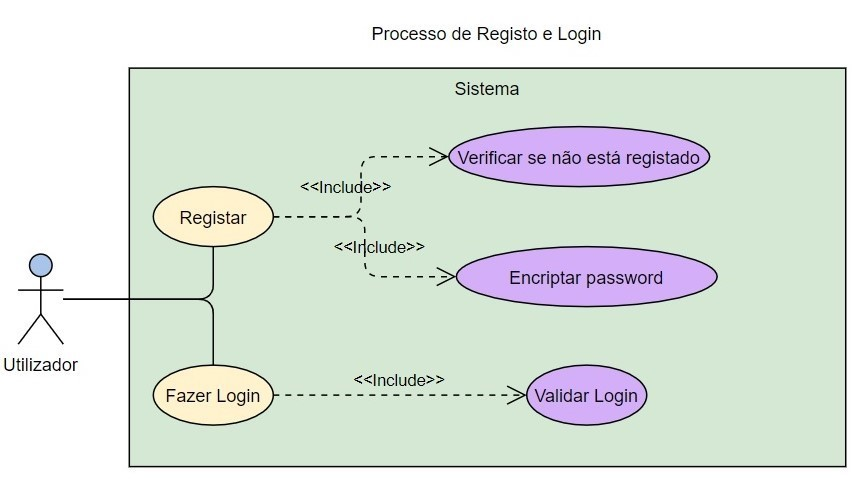
\includegraphics[scale=0.8]{Processo_Registo_Login.jpg}
    \caption[Diagrama de casos de uso: processo de registo e \emph{Login}]{Diagrama de casos de uso: processo de registo e \emph{Login}}
    \label{fig::casos-uso-regis}
\end{figure}

\begin{figure}[!htbp]
    \centering
    %\includegraphics[scale=0.8]{uso-homepage}
    \caption[Diagrama de casos de uso: \emph{homepage}]{Diagrama de casos de uso: \emph{homepage}.}
    \label{fig::casos-uso-homepage}
\end{figure}

\begin{figure}[!htbp]
    \centering
    %\includegraphics[scale=0.8]{uso-propdesafio}
    \caption[Diagrama de casos de uso: processo de propor desafio e cifra de mensagem]{Diagrama de casos de uso: processo de propor desafio e cifra de mensagem.}
    \label{fig::casos-uso-propdesafio}
\end{figure}

\begin{figure}[!htbp]
    \centering
    %\includegraphics[scale=0.8]{uso-repdesafio}
    \caption[Diagrama de casos de uso: processo de responder a desafios]{Diagrama de casos de uso: processo de responder a desafios.}
    \label{fig::casos-uso-repdesafio}
\end{figure}

\begin{figure}[!htbp]
    \centering
    %\includegraphics[scale=0.8]{uso-hash}
    \caption[Diagrama de casos de uso: processo de propor desafios do tipo valor de hash]{Diagrama de casos de uso: processo de propor desafios do tipo valor de hash.}
    \label{fig::casos-uso-hash}
\end{figure}

\section{Diagrama do sistema}
\label{sec::engsoft:diagrama-sistema}

\begin{figure}[!htbp]
    \centering
    %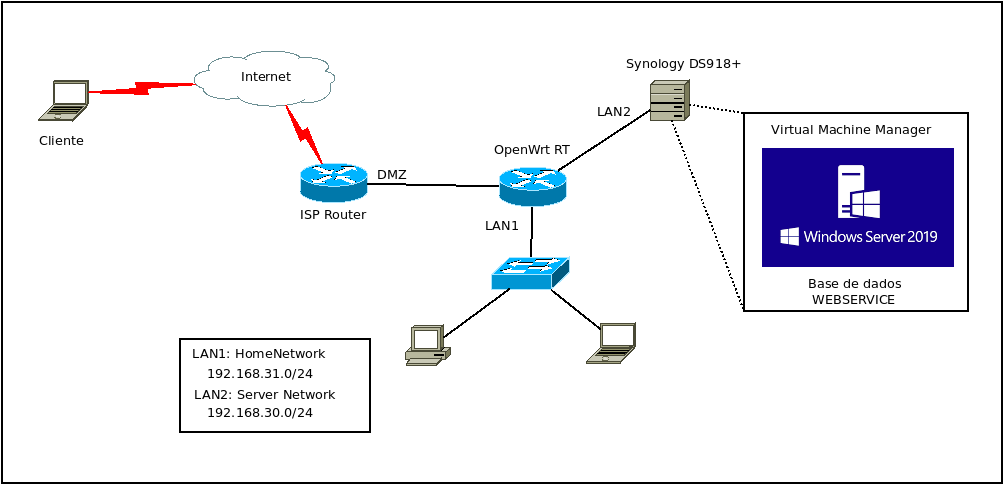
\includegraphics[scale=0.37]{DiagramaIdeal.png}
    \caption[Diagrama da arquitetura do sistema]{Diagrama da arquitetura do sistema}
    \label{fig::diagrama-sistema}
\end{figure}


\section{Conclusões}
\label{sec::engsoft:conclusao}

Na posse de um plano delineado segundo as práticas comuns da área da Engenharia de \textit{Software}, segue-se a fase de implementação, a qual deve seguir escrupulosamente os requisitos determinados e tem por base os casos de uso estudados. Por fim, o fluxo da aplicação deverá seguir o diagrama de atividades obtido por esta fase de estudo.

